\documentclass[12pt,a4paper]{article}
\usepackage{geometry}
\geometry{left=2.5cm,right=2.5cm,top=2.0cm,bottom=2.5cm}
\usepackage[english]{babel}
\usepackage{amsmath,amsthm}
\usepackage{amsfonts}
\usepackage[longend,ruled,linesnumbered]{algorithm2e}
\usepackage{fancyhdr}
\usepackage{ctex}
\usepackage{array}
\usepackage{listings}
\usepackage{color}
\usepackage{graphicx}
\usepackage[hidelinks]{hyperref}
% \usepackage[colorlinks=true, linkcolor=blue, urlcolor=blue]{hyperref}  % 自訂連結顏色並移除方框
% Add the following lines
\usepackage{fontspec}
\setmainfont{Sarasa Gothic TC}
\setCJKmainfont{Sarasa Gothic TC}

\begin{document}


\title{
  {
    \heiti Computer Graphics 第 1 次 Homework
  }
}


\date{2024/11/07}
\author{
  年級:{資工三}~~~~~~
  學號:{S11159005}~~~~~~
  姓名:{黃毓峰}~~~~~~
}

\maketitle
\newlength{\question}
\settowidth{\question}{XX}

\section*{\heiti \color{black}{電腦軟體系統簡介}}

\begin{itemize}
  \item Linux 6.11.5
  \item gcc - 14.2.1
  \item cmake - 3.30.5
  \item Wayland
  \item OpenGL - 4.6 
\end{itemize}

\section*{\heiti \color{black}{GLFW函式庫名稱與版本}}

\begin{itemize}
  \item GLFW - 3.4.0
\end{itemize}
\newpage
\section*{\heiti \color{black}{編譯後的執行成果}}
\begin{figure}[h]
  \centering
  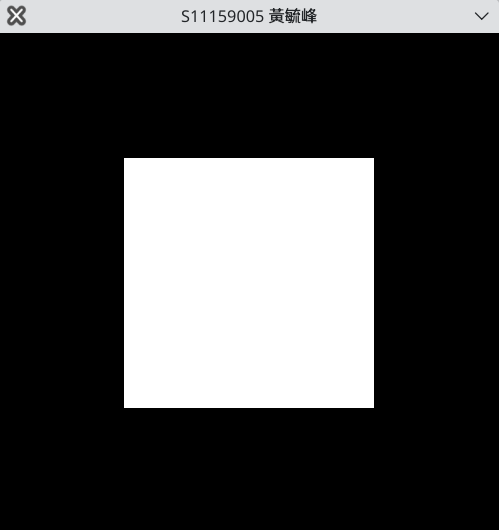
\includegraphics[width=0.8\textwidth]{img/hw1_result.png}
  \caption{執行結果}
\end{figure}


\section*{\heiti \color{black}{SourceCode}}
\sloppy
\noindent \url{https://github.com/IDK-Silver/NUTN-CSIE-Code/tree/main/ComputerGraphics/hw1}





\end{document}
